\documentclass{beamer}
\mode<presentation>
\usetheme{Montpellier}

\beamertemplatenavigationsymbolsempty
\pgfdeclareimage[]{logo}{escape-logo}
\logo{
\includegraphics{escape-logo}}

\title{}
\author{Dave Morris, Hendrik Heinl}
\institute{University of Edinburgh, CDS/CNRS}


\begin{document}

\begin{frame}
\titlepage
\end{frame}

\section*{Outline}
\begin{frame}{Outline}
\tableofcontents
\end{frame}

\section{What is the VO?}
\begin{frame}{What is the VO?}
A historical view: The Virtual Observatory (VO) is (or will be), a
\newline
\newline
\centerline{\textbf{comprehensive} set of}
\centerline{\textbf{data} and \textbf{services}}
\centerline{relevant to \textbf{astronomy}}
\centerline{accessible from \textbf{clients} of \textbf{your choice}}
\centerline{\textbf{regardless of where you are} and}
\centerline{\textbf{preserving} products of digital astronomy.}
\end{frame}

\begin{frame}{What it's (actually) not:}

A bundle of software used to work with data in astronomy. 
\newline
\newline
But of course you will find and use VO-client implementations in lots of
software like TOPCAT, Aladin, Splat-VO or PyVO. 

\end{frame}


\section{The challenge}

\begin{frame}{''FAIR''}
There's tens of thousands of data collections somewhere online,
and more should be.

To unlock the treasures hidden there, the data has to be
\begin{itemize}
\item \textbf{F}indable
\item \textbf{A}ccesible
\item \textbf{I}nteroperable
\item \textbf{R}eusable
\end{itemize}
\end{frame}

\section{Demo}

\begin{frame}{Demo time}

Let' see how all this works together.

\end{frame}



\section{Putting it together}

\begin{frame}{All at one glance:}

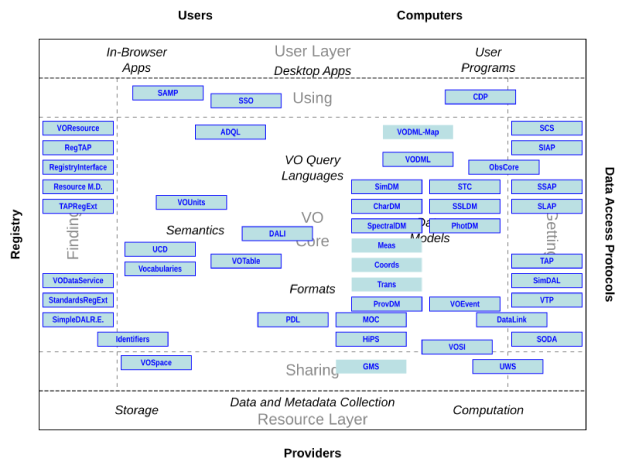
\includegraphics[width=\linewidth]{archdiag2.png}
\end{frame}



\end{document}
